\begin{name}
	{\tenchude}
	{ĐỀ ÔN TẬP CHƯƠNG I}
	{LỚP TOÁN THẦY PHÁT}
	{\thoigian}
\end{name}

\TN
\Opensolutionfile{ans}[ans/ansc101]
\begin{ex}%[Mức độ N]%[2D1N2-2]
	\immini{	Cho hàm số $y=f(x)$ có đồ thị như hình bên. Hàm số đạt cực đại tại
		\choice
		{$x=-3$}
		{\True $x=-2$}
		{$y=0$}
		{$y=4$}}{\begin{tikzpicture}[>=stealth]
			\draw [->] (-4,0)--(1.5,0);
			\draw [->] (0,-1)--(0,5);
			\draw (0,0) node[below right]{$O$};
			\draw (1.5,0) node[below]{$x$};
			\draw (0,5) node[below left]{$y$};
			\foreach \x in {-3,-2}{\draw (\x,-.1)--(\x,.1) node[below left,black]{$\x$};}
			\foreach \y in {4}{\draw [-] (-.1,\y)--(.1,\y) node[right,black]{$\y$};}
			\clip (-4,-1) rectangle (5,5);
			\draw [thick,samples=100] plot[domain=-5:5](\x,{(\x)^3+3*(\x)^2});
			\draw[dashed] (0,4) -- (-2,4) --(-2,0);
			\fill[black] (-2,4) circle(2pt);
			\draw (1,5) node[below right]{$f(x)$};
		\end{tikzpicture}}
	\loigiai{Từ hình vẽ, ta thấy hàm số $y=f(x)$ đạt cực đại tại điểm $x=-2$.}
\end{ex}

\begin{ex}%[2-D1B2-SO-5-2425]%[VN-MT-7, VM026]%[2D1N3-1]
	Cho hàm số $y=f\left( x \right)$ xác định và liên tục trên đoạn $\left[ -4;5 \right]$, có bảng biến thiên như hình sau
	\begin{center}
		
\begin{tikzpicture}
			\tkzTabInit[nocadre=true,lgt=1.0,espcl=3, deltacl=0.5]
			{$x$/0.7,$y’$/0.7,$y$/2}
			{$-4$,$-2$,$4$,$5$}
			\tkzTabLine{,+,0,-,0,+,}
			\tkzTabVar{-/$\dfrac{2}{3}$,+/$\dfrac{46}{3}$,-/$-\dfrac{62}{3}$,+/$-\dfrac{52}{3}$}
		\end{tikzpicture}
	\end{center}
	Gọi $M$, $N$ lần lượt là giá trị lớn nhất, giá trị nhỏ nhất của hàm số $y=f(x)$ xác định trên đoạn $[-4;5]$. Tính $M+N$?
	\choice
	{\True $-\frac{16}{3}$}
	{$-\frac{50}{3}$}
	{$2$}
	{$-20$}
	\loigiai{
		Dựa vào bảng biến thiên, ta có $M+N=\dfrac{46}{3}-\dfrac{62}{3}=-\dfrac{16}{3}$.
	}
\end{ex}

\begin{ex}%[2D1N5-5]
	\immini{Cho hàm số $f(x)$ có đạo hàm $f’(x)$ xác định, liên tục trên $\mathbb{R}$ và $f’(x)$ có đồ thị như hình vẽ bên. Khẳng định nào sau đây là đúng?
		\choice
		{Hàm số $f(x)$ đồng biến trên $(-\infty;1)$}
		{Hàm số $f(x)$ đồng biến trên $(-\infty;1)$ và $(1;+\infty)$}
		{\True Hàm số $f(x)$ đồng biến trên $(1;+\infty)$}
		{Hàm số $f(x)$ đồng biến trên $\mathbb{R}$}}
	{\begin{tikzpicture}[>=stealth,line join=round,line cap=round,font=\normalsize,scale=0.6]
			\draw[-stealth] (-1,0)--(0,0)node[above left]{$O$}--(3,0)node[below]{$x$};
			\draw[-stealth] (0,-3)--(0,3)node[left]{$y$};
			\draw (0,-2.5)--(1,0)--(2.5,2.5);
			\draw
			(1,0) node[below right]{$1$}
			;
		\end{tikzpicture}}
	\loigiai{
		Dựa vào đồ thị hàm số $f’(x)$, ta thấy $f’(x)>0,\forall x\in(1;+\infty)$ suy ra hàm số $f(x)$ đồng biến trên $(1;+\infty)$.}
\end{ex}

\begin{ex}%[2D1N5-1]
	\immini[thm]{Đồ thị hình bên là của một trong bốn hàm số sau. Hỏi đó là hàm số nào?
		\choice
		{$y=\dfrac{x^2+x-1}{x-1}$}
		{\True $y=\dfrac{x^{2}-x+1}{x-1}$}
		{$y=\dfrac{x^2-4x-1}{-x+1}$}
		{$y=\dfrac{x^2-3x-1}{-x+1}$}}{
		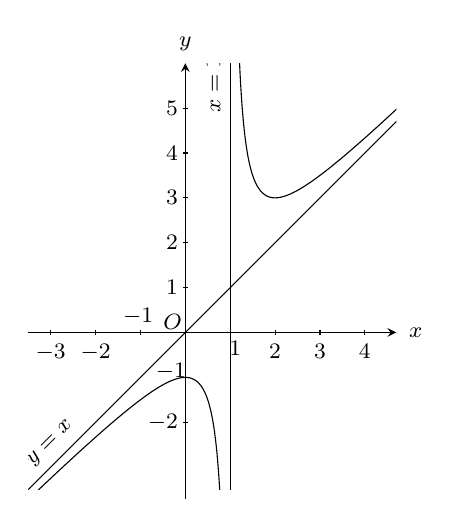
\begin{tikzpicture}[line cap=butt,line join=miter,>=stealth,scale=0.57,font=\footnotesize]
			\tikzset{declare function={xmin=-3.5;xmax=4.7;ymin=-3.5;ymax=6;},
				smooth,samples=450}
			\draw[->] (xmin,0)--(xmax,0) node[shift={(0:7pt)}]{$ x $};
			\draw[->] (0,ymin-.2)--(0,ymax) node[shift={(90:7pt)}]{$ y $};
			\fill (0,0) node[shift={(140:6pt)}]{$ O $};
			\clip (xmin,ymin) rectangle (xmax,ymax);
			\foreach \i in {-3,-2,2,3,4}{
					\draw(\i,1.5pt)--(\i,-1.5pt)node[below]{$\i$};}
			\foreach \j in {-2,1,2,3,4,5}{
					\draw(-1.5pt,\j)--(1.5pt,\j) node[left]{$\j$};}
			\draw(-1.5pt,-1)--(1.5pt,-1)node[shift={(160:6.5pt)}]{$-1$};
			\draw(1,-1.5pt)--(1,1.5pt)node[shift={(-75:7pt)}]{$1$};
			\draw(-1,-1.5pt)--(-1,1.5pt)node[shift={(100:5pt)}]{$-1$};
			\def\f(#1){((#1)^2-(#1)+1)/((#1)-1)}
			\def\a{-1}
			\def\b{0}
			\def\c{0.5}
			\def\d{1.5}
			\def\e{2}
			\def\g{3}
			\pgfmathsetmacro\fa{\f(\a)}
			\pgfmathsetmacro\fb{\f(\b)}
			\pgfmathsetmacro\fc{\f(\c)}
			\pgfmathsetmacro\fd{\f(\d)}
			\pgfmathsetmacro\fe{\f(\e)}
			\pgfmathsetmacro\fg{\f(\g)}
			\draw[samples=100] plot[domain=-5.3:0.9] (\x,{\f(\x)});
			\draw[samples=100] plot[domain=1.05:5.2] (\x,{\f(\x)});
			\draw[] (1,ymin)--(1,ymax) node [pos=0.95,sloped, above]{$x=1$};
			\draw[] (xmin,ymin)--(6,ymax) node [pos=0.08,sloped, above]{$y=x$};
		\end{tikzpicture}
	}
	\loigiai{
	}
\end{ex}

\begin{ex}%[2-D1B5-SO-16-2425]%[VN-MT-7, Dương Phước Sang]%[2D1H5-1]
	Cho bảng biến thiên của hàm số $y=f(x)$ như sau:
	\begin{center}
		
\begin{tikzpicture}
			\tikzset{double style/.append style={double distance=1.5pt}}
			\tkzTabInit[nocadre=true,lgt=1.2,espcl=4,deltacl=0.6]
			{$x$/0.6,$y'$/0.6,$y$/2}
			{$-\infty$,$1$,$+\infty$}
			\tkzTabLine{,-,d,-,}
			\tkzTabVar{+/$1$,-D+/$-\infty$/$+\infty$,-/$1$}
		\end{tikzpicture}
	\end{center}
	Hỏi đây là bảng biến thiên của hàm số nào trong các hàm số sau?
	\choice
	{$y=\dfrac{x-3}{x-1}$}
	{$y=\dfrac{-x+2}{x-1}$}
	{$y=\dfrac{x+2}{x+1}$}
	{\True $y=\dfrac{x+2}{x-1}$}
	\loigiai{
		Bảng biến thiên được cung cấp có đặc điểm:
		\begin{itemize}
			\item Đồ thị hàm số có đường tiệm cận đứng là $x=1$, loại $y=\dfrac{x+2}{x+1}$.
			\item Đồ thị hàm số có đường tiệm cận ngang là $y=1$, loại $y=\dfrac{-x+2}{x-1}$.
			\item $y'<0,\,\forall x \ne 1$, trong khi $\left(\dfrac{x-3}{x-1}\right)'=\dfrac{2}{(x-1)^2}>0,\,\forall x \neq 1$, loại $y=\dfrac{x-3}{x-1}$.
		\end{itemize}
		Chỉ có hàm số $y=\dfrac{x+2}{x-1}$ thỏa mãn các đặc điểm trên.
	}
\end{ex}

\begin{ex}%[BG-12NEW-4in1, Nguyen Huynh]%[2D1N4-1]
	\immini{
		Cho hàm số $y=\dfrac{2x^2}{x^2-1}$ có đồ thị là đường cong như hình vẽ bên. Số các đường tiệm cận đứng, tiệm cận ngang và tiệm cận xiên (nếu có) của đồ thị hàm số đã cho là	\choice{\True $4$}{ $2$}{ $3$}{$5$}}
	{	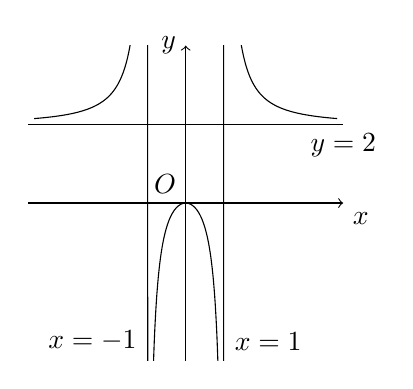
\begin{tikzpicture}[x=1cm,y=1cm,scale=.5]
			\draw[->] (-4,0)--(4,0)node[below right]{$x$};
			\draw[->] (0,-4)--(0,4)node[left]{$y$};
			\fill (0,0)node[above left]{ $O$};
			\draw (-4,2)--(4,2) node[below]{ $y=2$};
			\node at (-1,-4)[above left]{ $x=-1$};
			\node at (1,-4)[above right]{ $x=1$};
			\clip (-4,-4)rectangle(4,4);
			\draw[black,samples=150,smooth,domain=-3.85:3.85] plot(\x,{2*(\x)^(2)/((\x)^(2)-1)});
		\end{tikzpicture}
	}
	\loigiai{Đồ thị hàm số đã cho có tiệm cận đứng là các đường thẳng $x=-1$, $x=1$, tiệm cận ngang là đường thẳng $y=2$ và không có tiệm cận xiên}
\end{ex}

\begin{ex}%[Mức độ 3]%[2D1H2-1]
	Đồ thị của hàm số $y=x^3-3x^2-9x+1$ có hai điểm cực trị $A$ và $B$. Điểm nào dưới đây thuộc đường thẳng $AB$?
	\choice
	{$P (1;0)$}
	{$M (0;1)$}
	{\True $N(1;-10)$}
	{$Q (-1;10)$}
	\loigiai
	{
		Ta có $y'=3x^2-6x-9$.\\
		$y'=0\Leftrightarrow\hoac{&x=-1\Rightarrow y=6\\&x=3\Rightarrow y=-26.}$\\
		$\Rightarrow AB: y=-8x-2$
	}
\end{ex}

\begin{ex}%[De-chuan-hoa-so-1]%[Dương Quang]%[2D1N4-1]
	Đường tiệm cận ngang của đồ thị hàm số $y=\dfrac{2x-4}{-x+2}$ là
	\choice
	{ $y=2$}
	{ $x=2$}
	{$x=-2$}
	{\True$y=-2$}
	\loigiai{$\underset{x\to -\infty }{\mathop{\lim }}\,\dfrac{2x-4}{x+2}=-2$ và $\underset{x\to +\infty }{\mathop{\lim }}\,\dfrac{2x-4}{x+2}=-2$ nên đồ thị hàm số có tiệm cận ngang là $y=-2$.
	}
\end{ex}

\begin{ex}%[Mức độ H]%[2D1H3-4]
	Gọi $m$, $M$ lần lượt là giá trị nhỏ nhất, giá trị lớn nhất của hàm số $y=\sqrt{4-x^2}$. Tổng $m+M$ bằng
	\choice{\True $2$}{$0$}{$4$}{$1$}
	\loigiai{Tập xác định $\mathscr{D}=[-2;2]$.\\
	Ta có $y'=\dfrac{-x}{\sqrt{4-x^2} }\Rightarrow y'=0 \Leftrightarrow x = 0 \in [-2;2]$.\\
	Bảng biến thiên
	\begin{center}
		
\begin{tikzpicture}
			\tkzTabInit[nocadre=false, lgt=1.5,espcl=3.5]
			{$x$/1,$y'$/1,$y$/2}
			{$-2$,$0$,$2$}
			\tkzTabLine{,+,0,-, }
			\tkzTabVar{-/$0$,+/$2$,-/$0$/}
		\end{tikzpicture}
	\end{center}
	Dựa vào bảng biến thiên ta thấy $ \underset{[-2;2]}{\text{max}}y=2; \underset{[-2;2]}{\text{min}}y=0$.\\
	Vậy $m+M=0+2=2$.}
\end{ex}

\begin{ex}%[2D1H5-3]
	Cho hàm số $y=f(x)$ xác định, liên tục trên $\mathbb{R}$ và có bảng biến thiên sau
	\begin{center}
		
\begin{tikzpicture}
			\tkzTabInit[nocadre=false,lgt=0.7,espcl=2.1]
			{$x$ /0.6,$y'$ /0.6,$y$ /2}
			{$-\infty$,$-1$,$0$,$1$,$+\infty$}
			\tkzTabLine{,-,$0$,+,$0$,-,$0$,+,}
			\tkzTabVar{+/$-\infty$, -/$-1$,+/$0$,-/$-1$,+/$-\infty$}
		\end{tikzpicture}
	\end{center}
	Tìm tất cả các giá trị của tham số $m$ để phương trình $f(x)-1=m$ có đúng hai nghiệm.
	\choice
	{\True $m=-2,m>-1$}
	{$m=-2,m\ge -1$}
	{$-2<m<-1$}
	{$m>0,m=-1$}
	\loigiai{
	$f( x )-1=m\Leftrightarrow f( x )=m+1$. \\
	Dựa vào bảng biến thiên, để phương trình $f\left( x \right)-1=m$ có đúng hai nghiệm thì\\
	$\left[ \begin{aligned}
			 & m+1>0  \\
			 & m+1=-1 \\
		\end{aligned} \right.\Leftrightarrow \left[ \begin{aligned}
			 & m>-1  \\
			 & m=-2.
		\end{aligned} \right.$}
\end{ex}

\begin{ex}%[2-D1B3-SO-8-2425]%[VN-MT-7, Nguyễn Hồng Thạch]%[2D1H4-2]
	Tìm tất cả các giá trị thực của tham số $m$ để đồ thị hàm số $y=\dfrac{mx-8}{x+2}$ có hai đường tiệm cận.
	\choice
	{$m\neq 4$}
	{\True $m\neq -4$}
	{$m=4$}
	{$m=-4$}
	\loigiai{
		Ta có $x+2=0\Leftrightarrow x=-2$.\\
		Đồ thị hàm số đã cho có hai đường tiệm cận $\Leftrightarrow m\cdot(-2)-8\ne 0\Leftrightarrow m\neq -4$.}
\end{ex}

\begin{ex}%[De-chuan-hoa-so-15]%[Nguyễn Cường]%[2D1H3-6]
	Tại trường THPT Y, để giảm nhiệt độ trong các phòng học từ nhiệt độ ban đầu là $28^\circ C$, một hệ thống điều hòa làm mát được phép hoạt động trong $10$ phút. Gọi $T$ (đơn vị $^\circ C$) là nhiệt độ phòng ở phút thứ $t$ (tính từ thời điểm bật máy) được cho bởi công thức $T=-0{,}008t^3-0{,}16t+28$ $\left(t \in \left[0;10\right]\right)$. Nhiệt độ thấp nhất trong phòng có thể đạt được trong khoảng thời gian $10$ phút đó gần đúng là
	\choice
	{$27{,}832^\circ C$}
	{\True $18{,}4^\circ C$}
	{$26{,}2^\circ C$}
	{$25{,}312^\circ C$}
	\loigiai{
	Ta có $T'=-0{,}024t^2-0{,}16 < 0 \quad \forall t \in [0;10]$.\\
	$\Rightarrow T \ge T(10)=18{,}4^\circ C$.\\
	Do đó, nhiệt độ thấp nhất phòng có thể đạt được trong khoảng thời gian $10$ phút đó là $18{,}4^\circ C$.
	}
\end{ex}

\begin{ex}%[2D1V5-5]
	\immini{
		Cho hàm số $y=f(x)$ xác định trên $\mathbb{R}$, hàm số $y=f'(x)$ liên tục trên $\mathbb{R}$ và có đồ thị như hình vẽ bên. Hàm số $g(x)=f\left(3-\mathrm{e}^{x}\right)$ đồng biến trên khoảng nào dưới đây.
		\choice
		{\True$(2; 5)$}
		{$(-1; 0)$}
		{$(0; 1)$}
		{$(1; 2)$}
	}
	{
		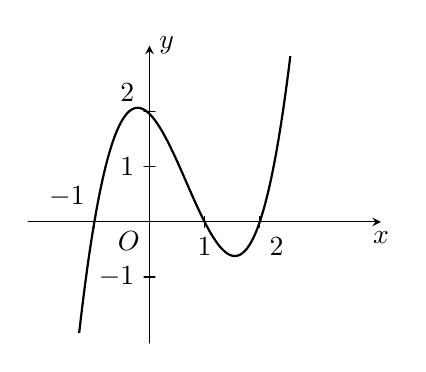
\begin{tikzpicture}[scale=0.7, line join=round, line cap=round, >=stealth]
			\tikzset{every node/.style={scale=1}}
			\def\xmin{-2}\def\xmax{4}\def\ymin{-2}\def\ymax{3}
			\draw[->] (\xmin-0.2,0)--(\xmax+0.2,0) node[below]{$x$};
			\draw[->] (0,\ymin-0.2)--(0,\ymax+0.2) node[right]{$y$};
			\draw (0,0) node[below left]{$O$};
			\foreach \x in {1}\draw (\x,0.1)--(\x,-0.1) node[below]{$\x$};
			\foreach \x in {-1}\draw (\x,-0.1)--(\x,0.1) node[above left]{$\x$};
			\foreach \x in {2}\draw (\x,0.1)--(\x,-0.1) node[below right]{$\x$};
			\foreach \y in {-1,1}\draw (0.1,\y)--(-0.1,\y) node[left]{$\y$};
			\foreach \y in {2}\draw (0.1,\y)--(-0.1,\y) node[above left]{$\y$};
			\clip (\xmin,\ymin) rectangle (\xmax,\ymax);
			\draw[thick,smooth,samples=200,domain=\xmin:\xmax] plot(\x,{0.98*((\x)^2-1)*((\x)-2)});
		\end{tikzpicture}
	}
	\loigiai{
		Ta có $g'(x)=-\mathrm{e}^{x} \cdot f'\left(3-\mathrm{e}^{x}\right)$.\\
		Để hàm số đồng biến thì \[-\mathrm{e}^{x} \cdot f'\left(3-\mathrm{e}^{x}\right)>0 \Leftrightarrow f'\left(3-\mathrm{e}^{x}\right)<0.\]
		Dựa vào đồ thị hàm số ta được
		\[
			f'\left(3-\mathrm{e}^{x}\right)<0 \Leftrightarrow \hoac{&3-\mathrm{e}^{x}<-1\\&1<3-\mathrm{e}^{x}<2} \Leftrightarrow \hoac{&\mathrm{e}^{x}>4\\&1<\mathrm{e}^{x}<2} \Leftrightarrow \hoac{&x>\ln 4\\&0<x<\ln 2.}
		\]
		Suy ra hàm số đồng biến trên $(0;\ln 2)$ và $(\ln 4;+\infty)$.\\
		Mà $(2;5)\subset (\ln 4;+\infty)$ nên hàm số đồng biến trên $(2;5)$.
	}

\end{ex}

\begin{ex}%[Mức độ 2]%[2D1H1-5]
	Cho chuyển động thẳng xác định bởi phương trình $S=t^3-3t^2+4t$, trong đó $t$ tính bằng giây $(s)$ và $S$ được tính bằng mét $~\mathrm{(m)}$. Gia tốc của chất điểm từ thời điểm $t=1$ đến thời điểm $t=2$ giây thay đổi như thế nào?
	\choice
	{Gia tốc tăng rồi giảm}
	{Gia tốc giảm}
	{\True Gia tốc tăng}
	{Gia tốc không thay đổi}
	\loigiai
	{
		Vận tốc của chất điểm là $v=s'=3t^2-6t+4$.\\
		Gia tốc của chất điểm là $a=v'=6t-6$.\\
		Vậy từ thời điểm $t=1$ giây đến $t=2$ giây, gia tốc của vật luôn tăng.
	}
\end{ex}

\begin{ex}%[BG12, Tran Tony]%[2D1H2-2]
	\immini{
		Cho hàm số $y=f(x)$ có bảng biến thiên như hình vẽ bên. Điểm cực tiểu của hàm số $y=f(3x)$ là
		\choice
		{\True $x=\dfrac{2}{3}$}
		{$x=2$}
		{$y=-3$}
		{$x=-\dfrac{2}{3}$}
	}{
		
\begin{tikzpicture}[font=\footnotesize, line join=round, line cap=round, >=stealth]
			\tkzTabInit[nocadre=false,lgt=1.2,espcl=2.2,deltacl=0.6]{$x$ /0.6,$f'(x)$ /0.6,$f(x)$ /2}{$-\infty$,$-1$,$2$,$+\infty$}
			\tkzTabLine{,+,0,-,+,}
			\tkzTabVar{-/$-\infty$,+/$4$,-/$-3$,+/$+\infty$}
		\end{tikzpicture}
	}
	\loigiai{
		Ta có $y'=3f'(3x)$, $f'(3x)=0\Leftrightarrow \hoac{&3x=-1\\&3x=2}\Leftrightarrow\hoac{&x=-\dfrac{1}{3}\\&x=\dfrac{2}{3}.}$\\
		Do $f'(x)$ và $3f'(3x)$ cùng dấu nên hàm số $y=f(3x)$ có điểm cực tiểu là $x=\dfrac{2}{3}$.
	}
\end{ex}

\begin{ex}%[2-D1B5-SO-14-2425]%[VN-MT-7, Đỗ Minh Phúc]%[2D1V3-6]
	Khi nuôi cá thí nghiệm trong hồ, một nhà khoa học đã nhận thấy rằng: nếu trên mỗi đơn vị diện tích của mặt hồ có $n$ con cá thì trung bình mỗi con cá sau một vụ cân nặng là $P(n)=800-20n$ (g). Hỏi phải thả bao nhiêu con cá trên một đơn vị diện tích của mặt hồ để sau một vụ thu hoạch được nhiều cá nhất?
	\choice
	{$19$}
	{\True $20$}
	{$21$}
	{$22$}
	\loigiai{
		Gọi $F(n)$ là hàm cân nặng của $n$ con cá sau vụ thu hoạch trên một đơn vị diện tích.\\
		Ta có $F(n)=(800-20n) \cdot n=800n-20n^2$.\\
		Để sau một vụ thu hoạch được nhiều cá nhất thì cân nặng của $n$ con cá trên một đơn vị điện tích của mặt hồ là lớn nhất.\\
		Bài toán trở thành tìm $n\in \mathbb{N}^*$ sao cho $F(n)$ đạt giá trị lớn nhất.\\
		Ta có $F'(n)=800-40n$.\\
		Cho $F'(n)=0 \Leftrightarrow 800-40n=0 \Leftrightarrow n=20$.\\
		Ta có bảng biến thiên
		\begin{center}
			
\begin{tikzpicture}
				\tkzTabInit[nocadre,lgt=1.2,espcl=2.5,deltacl=0.6]
				{$n$/0.6,$F'(n)$/0.6,$F(n)$/2}{$-\infty$,$20$,$+\infty$}
				\tkzTabLine{,+,0,-,}
				\tkzTabVar{-/$-\infty$,+/$8\,000$,-/$-\infty$}
			\end{tikzpicture}
		\end{center}
		Vậy phải thả $20$ con cá trên một đơn vị diện tích của mặt hồ để sau một vụ thu hoạch được nhiều cá nhất.
	}
\end{ex}

\begin{ex}%[BG12new-4in1, Trần Hoà]%[2D1H1-1]
	Cho hàm số $y=f(x)$ có  $f'(x)=(x+1)^2(x-1)^3(2-x), \forall x\in \mathbb{R}$. Hàm số $y=f(x)$ đồng biến trên khoảng nào dưới đây?
	\choice
	{\True $(1;2)$}
	{$(-\infty;-1)$}
	{$(-1;1)$}
	{$(2;+\infty)$}
	\loigiai
	{
		Dựa vào bảng xét dấu của $f'(x)$:
		\begin{center}
			
\begin{tikzpicture}
				\tkzTabInit[lgt=1.2,espcl=1.2]
				{$x$ /1, $f'(x)$ /1}
				{$-\infty$, $-1$,$1$, $2$, $+\infty$}
				\tkzTabLine{ ,-,z,-,z,+,z,-, }
			\end{tikzpicture}
		\end{center}
		ta suy ra hàm số $y=f(x)$ đồng biến trên $(1;2)$.
	}
\end{ex}

\begin{ex}%[Dự Án Giảng 12 4 in 1, Lê Văn Toàn]%[2D1N5-7]
	Đồ thị hàm số $y=\dfrac{2x+1}{x-1}$ cắt trục tung tại điểm có tung độ bằng
	\choice
	{$1$}
	{$-\dfrac{1}{2}$}
	{\True $-1$}
	{$2$}
	\loigiai{
		Gọi $M$ là giao điểm của đồ thị với trục tung, suy ra $x_M=0$.\\
		Thay vào biểu thức của đồ thị hàm số ta được $y_M=-1$.}
\end{ex}

\begin{ex}%[2D1H2-7]
	\immini{Đường dây điện $110KV$ kéo từ trạm phát (điểm $A$) trong đất liền ra Côn Đảo (điểm $C$). Biết khoảng cách ngắn nhất từ $C$ đến $B$ là $60$ km, khoảng cách từ $A$ đến $B$ là $100$ km, mỗi km dây điện dưới nước chi phí là $5000$ USD, chi phí cho mỗi km dây điện trên bờ là $3000$ USD. Hỏi điểm $D$ cách điểm $A$ bao nhiêu để mắc dây điện từ $A$ đến $D$ rồi từ $D$ đến $B$ chi phí đạt cực tiểu? (hình vẽ bên)
		\choice
		{$40$ km}
		{$50$ km}
		{\True $55$ km}
		{$45$ km}}{
		\begin{tikzpicture}[scale=1, font=\footnotesize, line join=round, line cap=round, >=stealth]
			\path
			(0,0) coordinate (A)
			(3,0) coordinate (D)
			(5,0) coordinate (B)
			(B)+(90:4) coordinate (C)
			;

			\draw (A)--(B)--(C)--(D) (A)--(C);

			\foreach \p/\r in {A/90,B/-120,D/-90,C/90}
			\fill (\p) circle (1.5pt) node[shift={(\r:3mm)}]{$\p$};
		\end{tikzpicture}
	}
	\loigiai{
		\immini{
			Đặt khoảng cách từ $D$ đến $B$ là $x$, $0\le x\le 100$. Khi đó khoảng cách từ $A$ đến $D$ là $100 - x$ km và khoảng cách từ $D$ đến $C$ là $\sqrt{x^2 + 3600}$ km. \\
			Chi thí cho việc kéo đường dây điện từ $A$ đến $D$ rồi đến $C$ được tính theo công thức
			\[f(x)=3000\left(100 - x\right) + 5000\sqrt{x^2 + 3600}=300000 - 3000x + 5000\sqrt{x^2 + 3600}.\]
			Ta xác định $x$ sao cho $f$ đạt cực tiểu. \\
			Ta có $f'(x)= - 3000 + \dfrac{5000x}{\sqrt{x^2 + 3600}}=0\Leftrightarrow x=45$.
		}
		{
			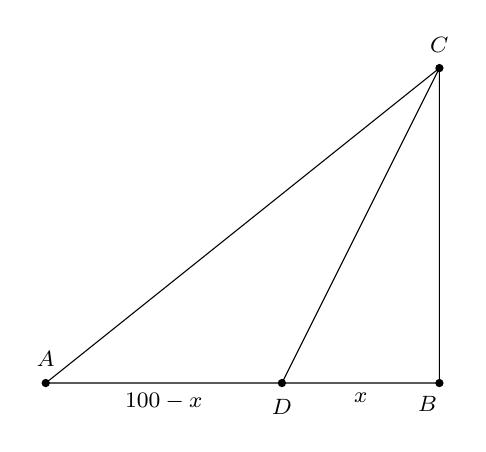
\begin{tikzpicture}[scale=1, font=\footnotesize, line join=round, line cap=round, >=stealth]
				\path
				(0,0) coordinate (A)
				(3,0) coordinate (D)
				(5,0) coordinate (B)
				(B)+(90:4) coordinate (C)
				;

				\draw (A)--node[midway,below]{$100-x$}(D)--node[midway,below]{$x$}(B)--(C)--(D) (A)--(C);

				\foreach \p/\r in {A/90,B/-120,D/-90,C/90}
				\fill (\p) circle (1.5pt) node[shift={(\r:3mm)}]{$\p$};
			\end{tikzpicture}
		}
		Bảng biến thiên
		\begin{center}
			
\begin{tikzpicture}
				\tkzTabInit[nocadre=false,lgt=1.2,espcl=2.5,deltacl=0.6]
				{$x$ /0.6,$f'(x)$ /0.6,$f(x)$ /2}
				{$0$,$45$,$100$}
				\tkzTabLine{,+,0,-,}
				\tkzTabVar{-/$f(0)$,+/$f(45)$,-/$f(100)$}
			\end{tikzpicture}
		\end{center}
		\noindent
		Dựa vào bảng biến thiên, hàm số $f(x)$ đạt cực tiểu khi $x=45$. Vậy khoảng cách cần tính để chi phí kéo dây là $55$ km.
	}
\end{ex}

\begin{ex}%[2D1H5-1]
	\immini{Người ta muốn chế tạo một chiếc hộp hình hộp chữ nhật có thể tích $500$ $\mathrm{cm}^3$. Chiều cao hộp phải là $2$ cm, các kích thước khác là $x, y$ với $x > 0$ và $y > 0$.
		Công thức xác định diện tích toàn phần $S(x)$ của chiếc hộp theo $x$ là
		\choice
		{$S(x)= 500+4 x-\dfrac{1000}{x}$}
		{\True $S(x)= 500+4 x+\dfrac{1000}{x}$}
		{$S(x)= 250+4 x+\dfrac{1000}{x}$}
		{$S(x)= 500+2 x+\dfrac{1000}{x}$}
	}{\begin{tikzpicture}[declare function={a=2;b=4;h=2;},line join=round,scale =0.8]
			\path (0,0) coordinate (B)
			(35:a) coordinate (A)
			(b,-1) coordinate (C)
			($(C)-(B)+(A)$) coordinate (D)
			($(A)+(90:h)$) coordinate (A')
			($(B)-(A)+(A')$) coordinate (B')
			($(C)-(A)+(A')$) coordinate (C')
			($(D)-(A)+(A')$) coordinate (D');
			\fill[orange!10] (B)--(B')--(A')--(D')--(D)--(C)--cycle;
			\draw ( B')--(B)--(C)--(D)--(D')--(A')--(B')--(C')--(D')  (C)--(C');
			\path (B)--(C)node[pos=0.5,sloped,black,below]{$x$};
			\path (C)--(D)node[pos=0.5,sloped,black,below]{$y$};
			\path (D)--(D')node[pos=0.5,sloped,black,below,scale=0.8]{$2$ cm};
			\draw[dashed]  (A')--(A)--(D)  (A)--(B);
		\end{tikzpicture}}
	\loigiai{
		\begin{itemize}
			\item Biểu thị $y$ theo $x$.\\
			      Ta có $500=x\cdot y \cdot 2 \Rightarrow y=\dfrac{250}{x}$.
			\item Diện tích toàn phần của chiếc hộp là
			      \[S(x)= 2\cdot 2\cdot x+2\cdot 2\cdot y+2\cdot x\cdot y= 500+4 x+\dfrac{1000}{x}.\]
		\end{itemize}
	}
\end{ex}

\begin{ex}%[2-D1B5-SO-16-2425]%[VN-MT-7, Dương Phước Sang]%[2D1H3-1]
	Giá trị lớn nhất của hàm số $f(x)=x^3-8x^2+16x-9$ trên đoạn $[1;3]$ là
	\choice
	{$\max\limits_{[1; 3]} f(x)=0$}
	{\True $\max\limits_{[1; 3]} f(x)=\dfrac{13}{27}$}
	{$\max\limits_{[1; 3]} f(x)=-6$}
	{$\max\limits_{[1; 3]} f(x)=5$}
	\loigiai{
		Hàm số $f(x)$ liên tục trên $[1;3]$.\\
		Ta có $f'(x)=3x^2-16x+16$; $f'(x)=0 \Leftrightarrow \hoac{&x=4 \notin (1;3)\\&x=\dfrac{4}{3}\in (1;3).}$\\
		$f(1)=0$; $f\left( \dfrac{4}{3} \right)=\dfrac{13}{27}$; $f(3)=-6$.\\
		Do đó $\max\limits_{x \in [1;3]} f(x)=f\left( \dfrac{4}{3} \right)=\dfrac{13}{27}$.
	}
\end{ex}

\begin{ex}%[2-D1B3-SO-7-2425]%[VN-MT-7, VM024]%[2D1N4-1]
	Cho hàm số $ y=f(x)$ có $\lim\limits_{x\to +\infty}f(x)=2$, $\lim\limits_{x\to -\infty}f(x)=+\infty$.
	\choice
	{Đồ thị hàm số đã cho có hai đường tiệm cận ngang}
	{Đồ thị hàm số đã cho có đúng một tiệm cận ngang là đường thẳng $x=2$}
	{\True Đồ thị hàm số đã cho có đúng một tiệm cận ngang}
	{Đồ thị hàm số đã cho không có tiệm cận ngang}
	\loigiai{
		Ta có $\lim\limits_{x\to +\infty}f(x)=2$. Do đó, đường thẳng $y=2$ là tiệm cận ngang của đồ thị hàm số $y=f(x)$.
	}
\end{ex}

\begin{ex}%[Mức độ N]%[2D1N3-1]
	Tìm giá trị lớn nhất của hàm số $y=\dfrac{3\sin x+2}{\sin x+1}$ trên đoạn $\left[0;\dfrac{\pi}{2}\right]$.
	\choice{\True $\dfrac{5}{2}$}{$\dfrac{11}{2}$}{$\dfrac{31}{2}$}{$2$}
	\loigiai{Đặt $t=\sin x$, $t \in [0;1]$.\\
		Xét hàm số $f(t)=\dfrac{3t+2}{t+1}$, $t \in [0;1].$\\Ta có $f'(t)=\dfrac{1}{(t+1)^2}>0$, $t\in [0;1]$.\\
		Vậy	$\underset{[0;1]}{\text{max}}f(t)=f(1)=\dfrac{5}{2}$.}
\end{ex}

\begin{ex}%[BG12new-4in1, Trần Hoà]%[2D1H1-2]
	\immini{Cho hàm số $y=f(x)$ xác định, liên tục trên $\mathbb{R}$ và có đạo hàm $f'(x)$. Biết rằng $f'(x)$ có đồ thị như hình vẽ bên. Mệnh đề nào sau đây đúng?
		\choice
		{\True Hàm số $y=f(x)$ nghịch biến trên khoảng $\left(0; + \infty\right)$}
		{Hàm số $y=f(x)$ nghịch biến trên khoảng $(- 3;-2)$}
		{Hàm số $y=f(x)$ đồng biến trên khoảng $\left(- \infty; 3\right)$}
		{Hàm số $y=f(x)$ đồng biến trên khoảng $(- 2; 0)$}}{\begin{tikzpicture}[>=stealth,line join=round,line cap=round,font=\footnotesize,scale=1]
			\draw[->] (-4.1,0)--(2.1,0) node[below left] {$x$};
			\draw[->] (0,-2.6)--(0,2.6) node[below left] {$y$};
			\draw[fill=black] (0,0) circle (1pt) node[above left] {$O$};
			\foreach \x in {-3,-2}
			\draw[thin] (\x,1pt)--(\x,-1pt) node [below left] {$\x$};
			\begin{scope}
				\clip (-4,-2.6) rectangle (2,2.6);
				\draw[samples=200,domain=-4:2,smooth,variable=\x] plot (\x,{(-(\x)-3)*((\x)+2)*((\x)^2)});
			\end{scope}
		\end{tikzpicture}}
	\loigiai{
		Từ đồ thị của hàm số, ta nhận thấy
		Với $\forall x\in \left(- 3; - 2\right)$, $f'(x)>0$ nên hàm số đồng biến.
		Với $\forall x\in \left(- \infty; - 3\right)$ và $(- 2; 0)$ và $\left(0; + \infty\right)$, $f'(x)<0$ nên hàm số nghịch biến.
		Vậy hàm số nghịch biến trên $\left(0; + \infty\right)$.}
\end{ex}

\begin{ex}%[Mức độ N]%[2D1N2-1]
	Hàm số nào dưới đây không có cực trị?
	\choice{$y=\dfrac{x^2+1}{x}$}{\True $y=\dfrac{2x-2}{x+1}$}{$y=x^2-2x+1$}{$y=-x^3+x+1$}
	\loigiai{Xét hàm số $y=\dfrac{2x-2}{x+1}\text{, } \forall x \ne-1$.\\ Ta có $y'=\dfrac{4}{(x+1)^2}>0\text{, } \forall x \ne -1$.\\
		Vậy hàm số $y=\dfrac{2x-2}{x+1}$ không cực trị.}
\end{ex}

\begin{ex}%[2D1N5-1]
	\immini[thm]{Bảng biến thiên ở hình bên là của một trong bốn hàm số sau đây. Hỏi đó là hàm số nào?
		\choice
		{$y=-x^3-2x^2+5$}
		{\True $y=x^3-3x^2+5$}
		{$y=-x^3-3x+5$}
		{$y=x^3+3x^2+5$}}{
		
\begin{tikzpicture}
			\tkzTabInit[nocadre=false, lgt=1.2, espcl=1.6]{$x$ /0.6,$f'(x)$ /0.6,$f(x)$ /1.5}{$-\infty$,$0$,$2$,$+\infty$}
			\tkzTabLine{,+,$0$,-,$0$,+,}
			\tkzTabVar{-/ $-\infty$/, +/$5$ , -/$1$  , +/$+\infty$/}
		\end{tikzpicture}}
	\loigiai{

	}
\end{ex}

\begin{ex}%[Mức độ 2]%[Dự án giảng new 4in1, Trần Quang Thạnh]%[2D1H1-4]
	Cho hàm số $y=f(x)$ có bảng biến thiên sau
	\begin{center}
		
\begin{tikzpicture}
			\tkzTabInit[nocadre=false,lgt=1.2,espcl=2.5]
			{$x$ /0.7,$f(x)$ /2}{$-\infty$,$0$,$4$,$+\infty$}
			\tkzTabVar{+/$+\infty$,-/$-5$,+/$-1$,-/$0$}
		\end{tikzpicture}
	\end{center}
	Bất phương trình $f(8x) < f(3x-185)$ có bao nhiêu nghiệm nguyên âm?
	\choice
	{$39$}
	{$38$}
	{$37$}
	{\True $36$}
	\loigiai{
		Ta thấy $f(x)$ nghịch biến trên khoảng $(0;+\infty)$.\\
		Với $x<0$, ta có $8x<0$ và $3x-185<0$, do đó
		\[f(8x) < f(3x-185) \Leftrightarrow 8x>3x-185 \Leftrightarrow x>-37.\]
		Vì $x$ nguyên âm nên $x\in\{-36;-35;\ldots;-1\}$.
	}
\end{ex}

\begin{ex}%[TEX NBV, Phạm Hoài]%[2D1N1-2]
	\immini[thm]{
		Biết hàm số $y=\dfrac{x+a}{x+1}$ ($a$ là số thực cho trước, $a\neq 1$ có đồ thị như hình bên). Mệnh đề nào dưới đây đúng?
		\choice
		{$y'<0, \,\forall x\neq -1$}
		{\True  $y'>0, \,\forall x\neq -1$}
		{$y'<0, \,\forall x\in \mathbb{R}$}
		{$y'>0, \,\forall x\in \mathbb{R}$}
	}{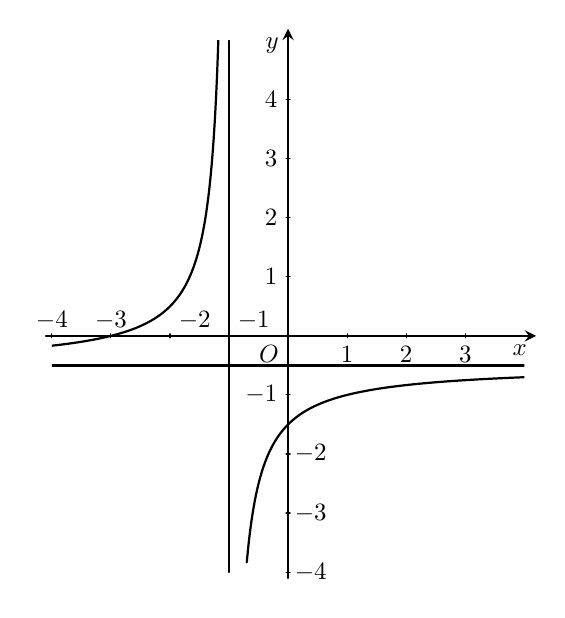
\begin{tikzpicture}[line join=round, line cap=round,>=stealth,thick,scale=0.75]
			\tikzset{every node/.style={scale=0.9}}
			\draw[->] (-4.1,0)--(4.2,0) node[below left] {$x$};
			\draw[->] (0,-4.1)--(0,5.2) node[below left] {$y$};
			\draw (0,0) node [below left] {$O$};
			\foreach \x/\nx in {1/1,2/2,3/3}
			\draw[thin] (\x,1pt)--(\x,-1pt) node [below] {$\nx$};
			\foreach \x/\nx in {-1/-1,-2/-2}
			\draw[thin] (\x,1pt)--(\x,-1pt) node [above right] {$\nx$};
			\foreach \x/\nx in {-4/-4,-3/-3}
			\draw[thin] (\x,1pt)--(\x,-1pt) node [above] {$\nx$};
			\foreach \y/\ny in {-1/-1,1/1,2/2,3/3,4/4}
			\draw[thin] (1pt,\y)--(-1pt,\y) node [left] {$\ny$};
			\foreach \y/\ny in {-4/-4,-3/-3,-2/-2}
			\draw[thin] (1pt,\y)--(-1pt,\y) node [right] {$\ny$};
			%\draw[dashed,thin](2,0)--(2,-6)--(0,-6);
			%\draw[dashed,thin] (1.01,-10)--(1.01,2);
			\begin{scope}
				\clip (-4,-4) rectangle (4,5);
				\draw[samples=200,domain=-5:-1.1,smooth,variable=\x] plot (\x,{(-1*(\x)-3)/(2*(\x)+2)});
				\draw[samples=200,domain=-.7:5,smooth,variable=\x] plot (\x,{(-1*(\x)-3)/(2*(\x)+2)});
				\draw (-1,-4)--(-1,5) (-5,-0.5)--(5,-0.5);
			\end{scope}
		\end{tikzpicture}}
	\loigiai{Dựa vào đồ thị, hàm số đồng biến trên từng khoảng xác định. Do đó $y'>0\, \forall x\ne -1$ suy ra $1-a>0\Rightarrow a<1$.
	}
\end{ex}

\begin{ex}%[Sách tham khảo, Mức độ H]%[Dự án giảng 12 - Trung Anh]%[2D1H2-4]
	Tìm tất cả các giá trị thực của tham số $m$ để hàm số $y=x^3-3(m+1)x^2+12mx+2019$ có hai điểm cực trị $x_1,\ x_2$ thỏa mãn $x_1+x_2+2x_1x_2=-8$.
	\choice
	{\True $m=-1$}
	{$m=2$}
	{$m=1$}
	{$m=-2$}
	\loigiai{
		Ta có $y'=3x^2-6(m+1)x+12m,\ y'=0\Leftrightarrow 3x^2-6(m+1)x+12m=0$. \\
		Hàm số có hai điểm cực trị $\Leftrightarrow \Delta '=9m^2-18m+9>0\Leftrightarrow m\ne 1$.\tagEX{1}
		Giả sử $x_1,\ x_2$ là hai nghiệm của phương trình $y'=0$, theo định lí Vi-ét ta có
		\[\heva{&x_1+x_2=-\dfrac{b}{a}=2(m+1)\\&x_1\cdot x_2=\dfrac{c}{a}=4m.}\]
		Do đó $x_1+x_2+2x_1\cdot x_2=-8\Leftrightarrow 2(m+1)+8m=-8\Leftrightarrow 10m=-10\Leftrightarrow m=-1$ thỏa mãn $(1)$.\\
		Vậy $m=-1$ là giá trị cần tìm của $m$.}
\end{ex}

\begin{ex}%[ĐỀ CHUẨN HÓA CHƯƠNG 1-GIẢI TÍCH 12]%[Huỳnh Đức Vũ]%[2D1V5-6]
	Cho hàm số $y=-x^3+3x^2+2$ có đồ thị $(C)$. Biết rằng, tại điểm $M$ thuộc $(C)$ tiếp tuyến của $(C)$ có hệ số góc lớn nhất. Tìm phương trình tiếp tuyến đó.
	\choice
	{\True $y=3x+1$}
	{$y=-3x+1$}
	{$y=-3x-1$}
	{$y=3x-1$}
	\loigiai{
		$y'=-3x^2+6x=-3(x-1)^2+3\leq 3$. \\
		Tiếp tuyến của $(C)$ có hệ số góc lớn nhất bằng $3$ tại điểm $M(1;4)$ có phương trình là
		$y=3(x-1)+4=3x+1$.}
\end{ex}

\begin{ex}%[Mức độ 3]giảng 12, Phạm Tiến Long]%[2D1V4-3]
	Tìm tham số $m$ để đồ thị hàm số $f(x)=\dfrac{x^2-mx+1}{x-2}$ có tiệm cận xiên cắt hai trục tọa độ $Ox$, $Oy$ tại hai điểm $A$, $B$ sao cho tam giác $OAB$  có diện tích bằng $8$.
	\choice
	{$m=2$ hoặc $m=6$}
	{\True $m=-2$ hoặc $m=6$}
	{$m=2$ hoặc $m=-6$}
	{$m=-2$ hoặc $m=-6$}
	\loigiai{	Hàm số đã cho có tập xác định $\mathscr{D}=\mathbb{R}\backslash\{-1\}$.\\
		Ta có $\begin{aligned}[t]
				a & =\lim\limits_{x \rightarrow+\infty} \dfrac{f(x)}{x}=\lim\limits_{x \rightarrow+\infty} \dfrac{x^2-mx+1}{x^2-2x}=1;                                                                \\
				b & =\lim\limits_{x \rightarrow+\infty}[f(x)-ax]=\lim\limits_{x \rightarrow+\infty}\left(\dfrac{x^2-mx+1}{x-2}-x\right)=\lim\limits_{x \rightarrow+\infty} \dfrac{(2-m)x+1}{x-2}=2-m.
			\end{aligned}$\\
		Ta cũng có $\lim\limits_{x \rightarrow-\infty} \dfrac{f(x)}{x}=1$; $\lim\limits_{x \rightarrow-\infty}[f(x)-x]=2-m$.\\
		Do đó, tiệm cận xiên của đồ thị hàm số là đường thẳng $d\colon y=x+2-m$.\\
		Đường thẳng $d$ cắt hai trục tọa độ tại hai điểm $A(0;2-m)$ và $B(m-2;0)$.\\
		Dễ thấy tam giác $OAB$ vuông cân tại $O$.\\
		Với điều kiện $m\ne 2$, ta có
		\begin{eqnarray*}
			& & \dfrac{1}{2}\cdot OA^2=8\\
			&\Leftrightarrow & \dfrac{1}{2} \cdot (2-m)^2=8\\
			&\Leftrightarrow & (2-m)^2=16\\
			&\Leftrightarrow & \hoac{&2-m=4\\&2-m=-4}\\
			&\Leftrightarrow & \hoac{&m=-2\text{ (thỏa điều kiện)}\\&m=6.\text{ (thỏa điều kiện)}}
		\end{eqnarray*}
		Vậy $m=-2$ hoặc $m=6$.
	}
\end{ex}

\begin{ex}%[Dự án TL12New-4in1-NCT]%[2D1V4-1]
	Cho hàm số $y=f(x)$ có bảng biến thiên như sau
	\begin{center}
		
\begin{tikzpicture}[>=stealth]
			\tkzTabInit[nocadre=false,lgt=1,espcl=3,deltacl=0.5]{$x$/.7 ,$y'$/.7,$y$/2}
			{$-\infty$ , $-2$ , $2$ , $+\infty$}
			\tkzTabLine{, + , $0$ , - , $0$ , + ,}
			\tkzTabVar{-/$-\infty$ , +/$3$ , -/$0$ , +/$+\infty$}
		\end{tikzpicture}
	\end{center}
	Đồ thị hàm số $y=\dfrac{1}{f(3-x)-2}$ có bao nhiêu tiệm cận đứng?
	\choice
	{$0$}
	{$2$}
	{\True $3$}
	{$1$}
	\loigiai{
		Ta thấy $f(x)=2$ có $3$ nghiệm $\Rightarrow$ đồ thị hàm số $y=\dfrac{1}{f(3-x)-2}$ có $3$ tiệm cận đứng.}
\end{ex}

\begin{ex}%[Dự án TL12New-4in1-NCT]%[2D1H4-2]
	Tìm tất cả các giá trị thực của tham số $m$ để đồ thị hàm số $y=\dfrac{mx+3}{\sqrt{mx^2-5}}$ có hai đường tiệm cận ngang.
	\choice
	{$m\geq 0$}
	{$m>\sqrt{5}$}
	{$m<0$}
	{\True $m>0$}
	\loigiai{
		Ta có $\lim\limits_{x\to+\infty}\dfrac{mx+3}{\sqrt{mx^2-5}}=\lim\limits_{x\to+\infty}\dfrac{m+\dfrac{3}{x}}{\sqrt{m-\dfrac{5}{x^2}}}$ và $\lim\limits_{x\to-\infty}\dfrac{mx+3}{\sqrt{mx^2-5}}=\lim\limits_{x\to-\infty}\dfrac{m+\dfrac{3}{x}}{-\sqrt{m-\dfrac{5}{x^2}}}$.\\
		Để đồ thị hàm số $y=\dfrac{mx+3}{\sqrt{mx^2-5}}$ có hai đường tiệm cận ngang thì $m>0$.\\
		Khi đó hai đường tiệm cận ngang là $y=\pm\sqrt{m}$.}
\end{ex}

\begin{ex}%[Mức độ 2]giảng 12, Phạm Tiến Long]%[2D1H4-3]
	Gọi $d$ là tiệm cận xiên của đồ thị hàm số $f(x)=2x-4+\dfrac{1}{3x+4}$. Giao điểm của $d$ với trục tung là
	\choice
	{$M(2;0)$}
	{$N(-2;0)$}
	{$P(0;4)$}
	{\True $Q(0;-4)$}
	\loigiai{
		Hàm số đã cho có tập xác định là $\mathbb{R}\backslash \left\{-\dfrac{4}{3}\right\}$.\\
		Ta có $\lim\limits_{x\to +\infty}[f(x)-(2x-4)]=0$ và $\lim\limits_{x\to -\infty}[f(x)-(2x-4)]=0$.\\
		Do đó, đồ thị hàm số có tiệm cận xiên là đường thẳng $d\colon y=2x-4$.\\
		Giao điểm của $d$ với trục tung là $Q(0;-4)$.
	}
\end{ex}
\begin{ex}%[CD12 - CTST, Mức độ 2] %[2D1H1-5]
	Chi phí sản xuất $x$ sản phẩm mỗi tháng của một công ty cho bởi hàm $\overline{C(x)}$ có bảng biến thiên như sau
	\begin{center}
		
\begin{tikzpicture}
			\tikzset{double style/.append style={double distance=2pt}}
			\tkzTabInit[lgt=1.2, espcl=2]
			{$x$/0.6,$\overline{C'}(x)$/0.6,$\overline{C}(x)$/1.5}{$0$,$1000$,$+\infty$}
			\tkzTabLine{,-,0,+,}
			\tkzTabVar{+/,-/$60$,+/$+\infty$}
		\end{tikzpicture}
	\end{center}
	Hỏi khi số sản phẩm mỗi tháng vượt qua giá trị bao nhiêu thì chi phí sản xuất bắt đầu tăng.
	\choice
	{\True $1\,000$}
	{$60$}
	{$500$}
	{$3\,60$}
	\loigiai{
		Từ bảng biến thiên ta thấy khi mỗi tháng xưởng sản xuất vượt quá $1\,000$ sản phẩm thì chi phí trung bình  sản xuất một sản phẩm thấp bắt đầu tăng.
	}
\end{ex}
\Closesolutionfile{ans}
\TL
\begin{ex}%[SGK12-CTST, Mức độ 2]%[2D1H2-1]
	Xét sự biến thiên và các điểm cực trị của hàm số $g(x)=\dfrac{x^2+x+4}{x+1}$.
	\loigiai{
		Tập xác định $\mathscr{D}=\mathbb{R}\setminus \{-1\}$.\\
		Ta có $g(x)=x+\dfrac{4}{x+1} \Rightarrow g'(x)=1-\dfrac{4}{(x+1)^2}=\dfrac{x^2+2x-3}{(x+1)^2}$;\\
		$g'(x)=0 \Leftrightarrow x^2+2x-3=0 \Leftrightarrow \hoac{& x=-3\\& x=1.}$\\
		Bảng biến thiên
		\begin{center}
			
\begin{tikzpicture}
				\tkzTabInit[nocadre=false,lgt=1.2,espcl=2.5,deltacl=0.6]
				{$x$ /0.6,$g'(x)$ /0.6,$g(x)$ /2}
				{$-\infty$,$-3$,$-1$,$1$,$+\infty$}
				\tkzTabLine{,+,$0$,-,d,-,$0$,+,}
				\tkzTabVar{-/$-\infty$,+/$-5$,-D+/$-\infty$/$+\infty$,-/$3$,+/$+\infty$}
			\end{tikzpicture}
		\end{center}
		Vậy hàm số đồng biến trên mỗi khoảng $(-\infty;-3)$ và $(1;+\infty)$; nghịch biến trên mỗi khoảng $(-3;-1)$ và $(-1;1)$. Hàm số đạt cực đại tại $x=-3$, $y_{\text{CĐ}}=g(-3)=-5$; và hàm số đạt cực tiểu tại $x=1$, $y_{\text{CT}}=g(1)=3$.
	}
\end{ex}
\begin{ex}%[2-D1B4-SO-10-2425]%[VN-MT-7, VM012]%[2D1V5-8]
	Giả sử chi phí cho xuất bản $x$ cuốn tạp chí (gồm: lương cán bộ, công nhân viên, giấy in,\ldots) được cho bởi công thức
	$C(x)=0{,}0\,001x^2-0{,}2x+10\,000$,
	trong đó $C(x)$ được tính theo đơn vị là vạn đồng ($1$ vạn đồng $=$ 10\,000 đồng). Chi phí phát hành cho mỗi cuốn là $4$ nghìn đồng. Tỉ số $M(x)=\dfrac{T(x)}{x}$ được gọi là chi phí trung bình cho một cuốn tạp chí khi xuất bản $x$ cuốn và tổng chi phí $T(x)$ (xuất bản và phát hành) cho $x$ cuốn tạp chí. Tìm chi phí trung bình thấp nhất cho một cuốn tạp chí là bao nhiêu vạn đồng, biết rằng nhu cầu hiện tại xuất bản không quá 30\,000 cuốn?
	% \shortans{2{,}2}
	\loigiai{
	Chi phí phát hành cho mỗi cuốn là $4$ nghìn đồng, tức là $0{,}4$ vạn đồng.\\
	Suy ra chi phí phát hành cho $x$ cuốn là $0{,}4x$ (vạn đồng).\\
	Theo đề bài, ta có tổng chi phí xuất bản và phát hành cho $x$ cuốn tạp chí là\\
	$T(x)=C(x)+0{,}4x=0{,}0\,001x^2+0{,}2x+10\,000$, với $x > 0$.\\
	Ta có $f(x)=M(x)=\dfrac{T(x)}{x}=0{,}0\,001x+0{,}2+\dfrac{10\,000}{x}$.\\
	Xét hàm số $f(x)=0{,}0\,001x+0{,}2+\dfrac{10\,000}{x}$, với $0< x\le 30\,000$.\\
	$f'(x)=0{,}0\,001-\dfrac{10\,000}{x^2}=\dfrac{0{,}0\,001x^2-10\,000}{x^2}$, $f'(x)=0\Leftrightarrow x=10\,000$ (do $x>0$).\\
	$\lim\limits_{x\to 0^+} f(x)=+\infty$.\\
	Bảng biến thiên:
	\begin{center}
		
\begin{tikzpicture}[>=stealth]
			\tkzTabInit[nocadre=true,lgt=1.2,espcl=2.5,deltacl=0.6]{$x$/.7 ,$f'(x)$/.7,$f(x)$/2}
			{$0$ , $10\,000$ , $30\,000$}
			\tkzTabLine{ , - , $0$ , + , }
			\tkzTabVar{+/$+\infty$ , -/$f(10\,000)$ , +/$f(30\,000)$}
		\end{tikzpicture}
	\end{center}
	Dựa vào bảng biến thiên, ta thấy giá trị của $M(x)$ nhỏ nhất khi $x=10\,000$.\\
	Do đó, số lượng tạp chí cần xuất bản sao cho chi phí trung bình thấp nhất là $x=10\,000$ (cuốn).\\
	Vậy chi phí trung bình cho một cuốn tạp chí khi xuất bản $10\,000$ cuốn là $M(10\,000)=2{,}2$ (vạn đồng).
	}
\end{ex}
\begin{ex}%[2-D1B1-SO-1-2425]%[VN-MT-7, Nguyễn Cao Cường]%[2D1C2-7]
	\immini[thm]{Người ta muốn thiết kế một lồng nuôi cá có bề mặt hình chữ nhật bao gồm phần mặt nước có diện tích bằng $54$ m$^2$ và phần đường đi xung quanh có thiết kế như hình vẽ (đơn vị: mét). Khi kích thước $a$ thay đổi trong khoảng $(3;+\infty)$ thì giá trị hàm số mô tả diện tích lối đi theo kích thước $a$ sẽ giảm đến giá trị $S_0$ rồi tăng lên. Xác định giá trị $S_0$.
	}
	{\begin{tikzpicture}[>=stealth,line join=round,line cap=round,font=\footnotesize,scale=0.75]
			\path
			(0,0) coordinate (A)
			(5,0) coordinate (B)
			(0,4) coordinate (D)
			($(D)+(B)-(A)$) coordinate (C)
			($(B)+(-0.5,0)$) coordinate (M)
			($(B)+(0,0.5)$) coordinate (N)
			($(A)+(1,0)$) coordinate (H)
			($(A)+(0,0.5)$) coordinate (T)
			($(C)+(-0.5,0)$) coordinate (Q)
			($(C)+(0,-0.5)$) coordinate (P)
			($(D)+(1,0)$) coordinate (R)
			($(D)+(0,-0.5)$) coordinate (S)
			($(T)+(H)-(A)$) coordinate (A')
			($(M)+(N)-(B)$) coordinate (B')
			($(Q)+(P)-(C)$) coordinate (C')
			($(R)+(S)-(D)$) coordinate (D')
			($(D)+(0,0.5)$) coordinate (x)
			($(C)+(0,0.5)$) coordinate (y)
			($(D)+(-0.5,0)$) coordinate (u)
			($(A)+(-0.5,0)$) coordinate (v)
			($(A)+(0,-0.5)$) coordinate (x')
			($(H)+(0,-0.5)$) coordinate (y')
			($(M)+(0,-0.5)$) coordinate (u')
			($(B)+(0,-0.5)$) coordinate (v')
			($(C)+(0.5,0)$) coordinate (x'')
			($(P)+(0.5,0)$) coordinate (y'')
			($(N)+(0.5,0)$) coordinate (u'')
			($(B)+(0.5,0)$) coordinate (v'')
			;
			\draw[fill=cyan!20!brown](A)--(B)--(C)--(D)--(A);
			\draw[fill=cyan!90!blue](A')--(B')--(C')--(D')--(A');
			\draw(D)--(x) (C)--(y)(D)--(u)(A)--(v)(A)--(x')(H)--(y')(M)--(u')(B)--(v')(C)--(x'') (P)--(y'') (N)--(u'') (B)--(v'');
			\draw[<->] (x)--(y)node[pos=0.5,above]{$a$};
			\draw[<->] (u)--(v)node[pos=0.5,left]{$b$};
			\draw[<->] (x')--(y')node[pos=0.5,below]{$2$};
			\draw[<->] (u')--(v')node[pos=0.5,below]{$1$};
			\draw[<->] (u'')--(v'')node[pos=0.5,right]{$1$};
			\draw[<->] (x'')--(y'')node[pos=0.5,right]{$1$};
		\end{tikzpicture}}
	% \shortans{42}
	\loigiai{
		Gọi $x$, $y$ lần lượt là độ dài, rộng của mặt nước. Điều kiện $x$, $y>0$.\\
		Phần mặt nước có diện tích bằng $54$ m$^2$ nên ta có $xy=54$. \quad\quad $(*)$\\
		Theo đề bài ta có $x=a-3$, $y=b-2$.\\
		Từ $(*)$ suy ra \[(a-3)(b-2)=54\Rightarrow b=\dfrac{54}{a-3}+2=\dfrac{2a+48}{a-3}.\]
		Diện tích lối đi là
		\allowdisplaybreaks
		\begin{eqnarray*}
			S(a)&=&a\cdot b-x\cdot y\\
			&=&ab-54\\
			&=&a\cdot \dfrac{2a+48}{a-3}-54\\
			&=&\dfrac{2a^2+48a}{a-3}-54.
		\end{eqnarray*}
		$S'(a)=\dfrac{2a^2-12a-144}{\left(a-3\right)^2}$.\\
		Xét $S'(a)=0\Leftrightarrow \hoac{&a=-6\\&a=12.}$\\
		Bảng biến thiên
		\begin{center}
			
\begin{tikzpicture}
				\tkzTabInit[nocadre=true,lgt=1.2,espcl=4,deltacl=0.5]
				{$a$ /0.7,$S'(a)$ /0.7,$S(a)$ /2}
				{$3$,$12$,$+\infty$}
				\tkzTabLine{,-,$0$,+,}
				\tkzTabVar{+/$+\infty$,-/$42$,+/$+\infty$}
			\end{tikzpicture}
		\end{center}
		Vậy $S_0=42$.
	}
\end{ex}
\begin{ex}%[Dự Án Giảng 12 4 in 1, Lê Văn Toàn]%[2D1C5-6]
	Cho hàm số $y=\dfrac{1}{4}x^4-\dfrac{7}{2}x^2$ có đồ thị $(C)$. Tiếp tuyến tại điểm $A$ thuộc $(C)$ cắt $(C)$ tại hai điểm phân biệt $M\left(x_1;y_1\right)$, $N\left(x_2;y_2\right)$ ($M$, $N$ khác $A)$ thỏa mãn $y_1-y_2=6\left(x_1-x_2\right)$. Các điểm $A$ thỏa mãn có tổng các hoành độ là
	% \shortans{$-3$}
	\loigiai{
		Gọi $A\left(x_0;y_0\right)\in\,(C)$ là tọa độ tiếp điểm của phương trình tiếp tuyến.\\
		Ta có hệ số góc $k=y'\left(x_0\right)=x_0^3-7x_0$.\\
		Phương trình tiếp tuyến $y=k\left(x-x_0\right)+y_0=\left(x_0^3-7x_0\right)\left(x-x_0\right)+y_0$.\\
		Ta có
		\begin{eqnarray*}
			&&y_1-y_2=6\left(x_1-x_2\right)\\
			&\Leftrightarrow& k\left(x_1-x_0\right)+y_0-\left[k\left(x_2-x_0\right)+y_0\right]=6\left(x_1-x_2\right)\\
			&\Leftrightarrow& k\left(x_1-x_2\right)=6\left(x_1-x_2\right)\\
			&\Leftrightarrow& k=6\\
			&\Leftrightarrow& x_0^3-7x_0=6\\
			&\Leftrightarrow& x_0^3-7x_0-6=0\\
			&\Leftrightarrow& \hoac{&x_0=3\Rightarrow y_0=-\dfrac{45}{4}\\&x_0=-1\Rightarrow y_0=-\dfrac{13}{4}\\&x_0=-2\Rightarrow y_0=-10.}
		\end{eqnarray*}
		Khi đó các phương trình tiếp tuyến tương ứng là
		\[\hoac{&d_1\colon y=6(x-3)-\dfrac{45}{4}=6x-\dfrac{117}{4}\\&d_2\colon y=6(x+1)-\dfrac{13}{4}=6x+\dfrac{11}{4}\\&d_3\colon y=6(x+2)-10=6x+2.}\]
		Phương trình hoành độ giao điểm của $(C)$ với các tiếp tuyến là
		\[\hoac{&\dfrac{1}{4}x^4-\dfrac{7}{2}x^2-6x+\dfrac{117}{4}=0\text{ (có 1 nghiệm nên không thỏa)}\\&\dfrac{1}{4}x^4-\dfrac{7}{2}x^2-6x-\dfrac{11}{4}=0\text{ (có 3 nghiệm nên thỏa mãn)}\\&\dfrac{1}{4}x^4-\dfrac{7}{2}x^2-6x-2=0\text{ (có 3 nghiệm nên thỏa mãn).}}\]
		Do đó tổng các hoành độ điểm các tiếp điểm là $-1-2=-3$.
	}
\end{ex}
% \begin{indapan}
% 	{ans/ansc1l4}
% \end{indapan}

